\documentclass[conference]{IEEEtran}
\usepackage{cite}
\usepackage{array}
\usepackage{graphicx}
\usepackage{amsthm}
\usepackage{amsmath}
\usepackage{amssymb}
\usepackage{mathrsfs}
% \usepackage{minted}
\usepackage{listings}
\usepackage{color} 						% red, green, blue, yellow, cyan, magenta, black, white

\usepackage{float} %used to force figures in a position
\hyphenation{op-tical net-works semi-conduc-tor}

\theoremstyle{definition}
\newtheorem{definition}{Definition}[section]

\begin{document}
\title{Clasificaci\'{o}n de ECG usando Redes Neuronales}

\author{\IEEEauthorblockN{J. Agust\'{i}n Barrachina}
	\IEEEauthorblockA{Miembro Estudiantil IEEE\\
		Instituto Tecnol\'{o}gico de Buenos Aires\\}}
\maketitle

% \tableofcontents
% \newpage

\begin{abstract}
	Se clasificaron latidos de un segmento de se\~{n}al de un electrocardiograma seg\'{u}n el tipo de arritmia. El algoritmo utilizado fue un perceptr\'{o}n multicapa usando backpropagation como clasificador. Se utilizaron PCA y SOM para reducir la dimensionalidad de los datos.
\end{abstract}

\section{Introducci\'{o}n}

El trabajo consisti\'{o} en clasificar los latidos de un segmento de una se\~{n}al de electrocardiograma de dos canales de 21 horas de duraci\'{o}n seg\'{u}n el tipo de arritmia.

El objetivo fue crear y entrenar un sistema que pueda reconocer y clasificar los distintos tipos de latidos.

\section{Data Set}

Se utilizaron las grabaciones de "MIT-BIH Long Term Database" \cite{MIT-BIH} disponible en el repositorio PhysioNet \cite{PHYSIONET}.

La grabaci\'{o}n incluye anotaciones que identifican la posici\'{o}n y tipo de cada uno de los latidos presentes en la misma.

La grabaci\'{o}n se identificar\'{a} por el n\'{u}mero 14172, y el identificador de la base de datos es "ltdb" (\underline{L}ong \underline{T}erm \underline{D}ata\underline{B}ase).
La misma presenta principalmente 4 tipos de latidos:

\begin{itemize}
	\item \textbf{Normales}. Identificados por la letra 'N'.
	\item \textbf{Ventriculares prematuros} Identificados por la letra 'V'.
	\item \textbf{Supraventriculares prematuros} Identificados por la letra 'S'.
	\item \textbf{Nodales prematuros} Identificados por la letra 'J'.
\end{itemize}

Para el tratamiento de los datos se utliz\'{o} la librer\'{i}a de python "wfdb" \cite{WFDB}.

A continuaci\'{o}n se muestran la cantidad de latidos de cada tipo que poseen los datos.

\begin{lstlisting}[frame=single]
('Numero de latidos: ', 66409)
set(['a', 'F', 'J', 'N', 'S', 'V', '~'])
a :  1
F :  1
J :  148
N :  58323
S :  1003
V :  6530
~ :  407
\end{lstlisting}

\subsection{Reducci\'{o}n de Dimensionalidad}

Se usaron dos t\'{e}cnicas distintas para reducir la dimensi\'{o}n de los datos y as\'{i} acelerar y facilitar las operaciones de la red neuronal.

La primera t\'{e}cnica fue la utilizaci\'{o}n de \textit{\underline{P}rincipal \underline{C}omponen \underline{A}nalysis} (PCA). La teor\'{i}a del mismo no se desarrollar\'{a} en \'{e}ste informe.

Otra t\'{e}cnica utilizada fue la implementaci\'{o}n de una red \textit{\underline{S}elf \underline{O}rganized \underline{M}ap} (SOM) que tampoco se desarrollar\'{a} en este informe.

Finalmente se decidi\'{o} por utilizar la implementaci\'{o}n del PCA por un motivo puramente de tiempo de ejecuci\'{o}n, ya que la red SOM requer\'{i}a mucho tiempo de c\'{o}mputo y no obten\'{i}a resultados perceptiblemente superiores a los de la red PCA. Se trunc\'{o} las dimensiones de PCA reduciendo los datos de cada latido de 250 a 32. En la figura \ref{fig_pca_reduction} se muestra un ejemplo de los datos originales contra los datos "filtrados".

\begin{figure}[H]
	\centering
	\includegraphics[width=9cm]{../out/PCAexample.png}
	\caption{Ejemplo de reducci\'{o}n de los datos utilizando PCA}
	\label{fig_pca_reduction}
\end{figure}

\section{Dise\~{n}o de la Red Neuronal}

Seg\'{u}n Rezaul Begg et al. \cite{NN_HEALTHCARE}, la t\'{e}cnica m\'{a}s com\'{u}nmente utilizada de Redes Neuronales hasta el d\'{i}a de la fecha en procesamiento de ECG es el perceptr\'{o}n multicapa (MLP) entrenada con backpropagation (Secci\'{o}n 2 Cap\'{i}tulo 3), por dicho motivo se utilizar\'{a} \'{e}ste mismo como el algoritmo para utilizar en \'{e}ste trabajo.

El mismo trabajo posee una tabla (figura \ref{tab_tabla_comparacion_tecnicas}) que presenta diferentes aplicaciones de redes neuronales en el \'{a}mbito de cardiolog\'{i}a. Lamentablemente ninguno de los casos es aplicable a nuestro caso ya que suelen ser diferenciaci\'{o}n entre si y no sobre la probabilidad de tener AMI. Sin embargo, la mayor\'{i}a de los casos usan una configuraci\'{o}n de MLP de una sola capa oculta con lo cual en este trabajo se utilizar\'{a} esa misma configuraci\'{o}n.
Normalmente adem\'{a}s se recomienda utilizar solo una capa ya que casi con seguridad no ser\'{a} necesario m\'{a}s capas.

\begin{figure}[H]
	\centering
	\includegraphics[width=8cm]{../out/ECG_table_techinques.png}
	\caption{Redes Neuronales Aplicadas en Cardiolog\'{i}a seg\'{u}n \cite{NN_HEALTHCARE}}
	\label{tab_tabla_comparacion_tecnicas}
\end{figure}

Si bien existen varios trabajos sobre la elecci\'{o}n de la cantidad de elementos re la red oculta como \cite{SIZE1} o \cite{SIZE2}, no existe una receta \'{u}nica e infalible sobre cu\'{a}ntos nodos darle a la capa oculta. Para elegirlos se utilizaron las siguientes reglas \textit{RoT} (Rule of Thumb) que se describir\'{a}n a continuaci\'{o}n.

\begin{enumerate}
	\item \textit{Errar por m\'{a}s y no por menos:} Unos nodos extra no es probable que causen da\~{n}o a la convergencia de la red, se los puede pensar como un exceso de capacidad. Mientras que usar pocos nodos pueden afectar a la convergencia. 
	\item \textit{Basado en la entrada y la salida:} Utilizar una cantidad de nodos que se encuentren entre la cantidad de nodos de la entrada y la cantidad de nodos de la salida. (Jeff Heaton autor de \textit{"Introduction to Neural Networks for Java"})
\end{enumerate}

Utilizando estas dos reglas se eligi\'{o} utilizar la expresi\'{o}n \( nodos_{hidden} = (nodos_{entrada} + nodos_{salida})/1.5\).

Para el algoritmo de aprendizaje se utiliz\'{o} una librer\'{i}a \cite{NIMBLENET} que implementa redes neurnales feed-forward (Redes Multicapa) permitiendo una variedad de algorimos de aprendizajes de backpropagation.

\subsection{Set de Entrenamiento}

En un primer momento se entrenaba la red con los primeros casos de latidos. Para dicho set de entrenamiento, el error aumentaba a medida que los datos estaban m\'{a}s alejados temporalmente de los mismos, es decir, si se tomaban los primeros 10 casos del set de datos para el entrenamiento, el conjunto de datos a partir del onceavo hasta el veinteavo mostraba grandes resultados, mientras que los datos rondando el n\'{u}mero mil pose\'{i}a resultados muy poco satisfactorios.

Para contrarrestar este problema se tomaron los datos de entrenamiento de forma aleatoria. \'{E}sto logr\'{o} mejorar mucho el desempe\~{n}o pero a coste de tener mayor varianza en los resultados. Adem\'{a}s el caso de seleccionar dos veces los mismos datos puede ocurrir con el c\'{o}digo actual.

\section{Overfitting}

Se utiliz\'{o} un test set para ir verificando la evoluci\'{o}n de la red. Como no se deseaba darle prioridad a ning\'{u}n latido sobre los dem\'{a}s se utiliz\'{o} la misma cantidad para cada categor\'{i}a. Siendo el m\'{a}ximo numero de latidos de la categor\'{i}a con menor cantidad de latidos 148. Se tom\'{o} 100 datos de cada categor\'{i}a como test set.

La implementaci\'{o}n de la red present\'{o} overfitting. Como se puede ver en los resultados listados a continuaci\'{o}n, el error del set de datos del test set comienza a incrementar.

\begin{lstlisting}[frame=single]
Error: 	0.290525167175 	Epoch: 1000
Error: 	0.252432576731 	Epoch: 2000
Error: 	0.233333077085 	Epoch: 3000
Error: 	0.226507241997 	Epoch: 4000
Error: 	0.227502496085 	Epoch: 5000
Error: 	0.230580316278 	Epoch: 6000
Error: 	0.233771065888 	Epoch: 7000
Error: 	0.236764878811 	Epoch: 8000
Error: 	0.239612203297 	Epoch: 9000
Error: 	0.242385089641 	Epoch: 10000
\end{lstlisting}

La librer\'{i}a utilizada \cite{NIMBLENET} permite el uso de dropout para poder reducir el overfitting. El resultado a continuaci\'{o}n muestra el caso para un dropout del 50\%.

\begin{lstlisting}[frame=single]
Error: 0.330238968525 	Epoch: 1000
Error: 0.254160001896 	Epoch: 2000
Error: 0.214160846981 	Epoch: 3000
Error: 0.193992225022 	Epoch: 4000
Error: 0.185100235993 	Epoch: 5000
Error: 0.180218777466 	Epoch: 6000
Error: 0.176489777988 	Epoch: 7000
Error: 0.173452841416 	Epoch: 8000
Error: 0.171893196978 	Epoch: 9000
Error: 0.172405423062 	Epoch: 10000
\end{lstlisting}

Se puede observar que el dropout mejor\'{o} notoriamente el overfitting haciendo que el mismo sea de pasados las 9000 iteraciones. Se realiz\'{o} entonces una simulaci\'{o}n de montecarlo para distintos valores de dropout a fin de verificar el valor \'{o}ptimo del mismo y comparar su impacto en el resultado. El resultado se muestra en la tabla \ref{tab_dropout_montecarlo}.

\begin{table}[h]
	\centering
	\caption{MSE para distintos valores de dropout}
	\label{tab_dropout_montecarlo}
	\begin{tabular}{ c c c }    
		\hline \\ 
		\textsc{Dropout} & \textsc{MSE} & \textsc{Epoch}    \\ 
		\hline 
		\\
		0\%		&  0.2233 \(\pm\) 0.0070 	& 5011 \(\pm\) 443 	\\
		50\% 	&  0.1973 \(\pm\) 0.0045 	& 7141 \(\pm\) 393 	\\
		60\%  	&  0.1946 \(\pm\) 0.0029 	& 7662 \(\pm\) 324	\\
		70\% 	&  0.1979 \(\pm\) 0.0038 	& 6639 \(\pm\) 1428 \\
		80\%  	&  0.1872 \(\pm\) 0.0033 	& 7310 \(\pm\) 483	\\
		90\%  	&  0.1953 \(\pm\) 0.0040 	& 6725 \(\pm\) 491 	\\
		\hline
	\end{tabular}
\end{table}

Se puede ver como a medida que aumenta el dropout, el error cuadr\'{a}tico medio se va reduciendo hasta llegar al 80\%, tras lo cual comienza a aumentar de vuelta. Se elige entonces un dropout de 80\% para este trabajo.

\subsection{Modificaci\'{o}n de la Librer\'{i}a: Early Stop}
Sin embargo el overfitting no se elimin\'{o} por completo y existe un n\'{u}mero \'{o}ptimo para el cual conviene no seguir entrenando la red. Por dicho motivo, se modific\'{o} la librer\'{i}a para poder realizar \textit{early stop}. 
La implementaci\'{o}n permite elegir la cantidad de iteraciones con un aumento del error antes de abandonar el entrenamiento (que se denominar\'{a} \textit{tolerancia del early stop}).  

En un principio se hizo que esas iteraciones fueran consecutivas exclusivamente, es decir, que el error aumente sin interrupci\'{o}n durante esa cantidad de iteraciones. \'{E}sto gener\'{o} que con valores muy altos de tolerancia, jam\'{a}s ocurriera el early stop.
\'{E}sto luego se cambi\'{o} para que la diferencia entre los \'{u}ltimos cambios haya sido superior a la tolerancia. 

Se realiz\'{o} una simulaci\'{o}n para obtener el valor que mejor consiga adecuarse al valor real del m\'{i}nimo error.

\begin{table}[h]
	\centering
	\caption{Tolerancia de Early Stop}
	\label{tab_early_stop_montecarlo}
	\begin{tabular}{ c c c }    
		\hline \\ 
		\textsc{Early Stop Tolerance} & \textsc{MSE error} &  \textsc{Epoch Error}   \\ 
		\hline 
		\\
		1	&  0.032274 \(\pm\) 0.002175 	& 6898 \(\pm\) 867 	\\
		5 	&  0.000329 \(\pm\) 0.000140 	& 4575 \(\pm\) 876 	\\
		10  &  0.000178 \(\pm\) 0.000153 	& 2795 \(\pm\) 1361 \\
		15  &  0.000002 \(\pm\) 0.000001 	& 386  \(\pm\) 168 	\\
		20  &  0.000001 \(\pm\) 4e-07 		& 561  \(\pm\) 308 	\\
		24  &  0.000001 \(\pm\) 5.4e-07 	& -46  \(\pm\) 218 	\\
		28  &  4.5e-07  \(\pm\) 1.5e-07 	& -253  \(\pm\) 144 \\
		30	&  2.6e-07	\(\pm\) 1e-07 		& -223  \(\pm\) 102 \\
		32  &  6.5e-07  \(\pm\) 2e-07 		& -389  \(\pm\) 107 \\
		34  &  0.000001 \(\pm\) 4e-07 		& -477  \(\pm\) 191 \\
		40	&  7.6e-07	\(\pm\) 1.4e-07 	& -306  \(\pm\) 131 \\
		\hline
	\end{tabular}
\end{table}

Se dej\'{o} el error de los epochs como diferencia bruta (y no su cuadrado) para poder observar como a partir de cierto punto, el algoritmo termina despu\'{e}s del m\'{i}nimo de la funci\'{o}n. \'{E}sto demuestra como una tolerancia baja de \textit{early stop} hace que el la red deje de entrenar antes de alcanzado el punto \'{o}ptimo mientras que colocar una tolerancia muy alta hace que el mismo termine mucho despu\'{e}s. Si se desea observar el error cuadr\'{a}tico se puede ver la figura \ref{fig_epoch_error}.

La figura \ref{fig_mse_error} muestra el MSE error que figura en la tabla \ref{tab_early_stop_montecarlo}. 

\begin{figure}[H]
	\centering
	\includegraphics[width=8cm]{../out/epoch.png}
	\caption{Error MSE de la cantidad de epochs realizados de m\'{a}s o de menos antes del early stop}
	\label{fig_epoch_error}
\end{figure}

\begin{figure}[H]
	\centering
	\includegraphics[width=8cm]{../out/mse_error.png}
	\caption{Error MSE conseguido con early stop contra el \'{o}ptimo de la iteraci\'{o}n}
	\label{fig_mse_error}
\end{figure}

\section{Implementaci\'{o}n de la Red} \label{sec_config}

La siguiente figura (figura \ref{fig_diagram}, levemente modificada de la figura 6 de \cite{NN_HEALTHCARE}) muestra el diagrama b\'{a}sico de la implementaci\'{o}n del proyecto.

\begin{figure}[H]
	\centering
	\includegraphics[width=8cm]{../out/diagrama.png}
	\caption{Diagrama general del proyecto}
	\label{fig_diagram}
\end{figure}

En primer lugar se extrae y se extraen varios vectores de dimensi\'{o}n 250 de cada caso de latido. 
Luego se reduce su dimensi\'{o}n utilizando PCA o SOM a una dimensi\'{o}n menor.
Finalmente se aplica la red multicapa obteniendo la salida \(y_i\) donde cada valor corresponde a una clasificaci\'{o}n posible (\(0 \le y_i \le 1\) que representa la probabilidad de que el latido corresponda a dicha clasificaci\'{o}n). 

\begin{itemize}
	\item Reducci\'{o}n de Dimensi\'{o}n usando PCA 32
	\item Configuraci\'{o}n 32 - 24 - 4
	\item Funci\'{o}n de activaci\'{o}n: Sigmoidea
	\item Cantidad de latidos de entrenamiento: 10
	\item Cantidad de latidos de test set: 100
	\item Dropout = 80\%
	\item Tolerancia Early Stop 30
\end{itemize}

\section{An\'{a}lisis de los Resultados} \label{sec_analisis_resultados}

Para analizar los resultados se usaron dos par\'{a}metros que se los denomin\'{o} \textit{aciertos} y los \textit{hallados}. 

El primero cuenta la cantidad de \textit{aciertos} de cada decisi\'{o}n, es decir, si se dijo que cierto numero de latidos corresponden a un categor\'{i}a, cu\'{a}ntos de ellos realmente eran de esa categor\'{i}a.

Por ejemplo, si encuentro 100 latidos ' N' y 90 de ellos lo eran, el porcentaje de aciertos ser\'{a} del 90\% lo cual parece ser un n\'{u}mero muy aceptable. Sin embargo, si se aliment\'{o} la red con 900 latidos, solo el 10\% fueron hallados, haciendo que el desempe\~{n}o de la red sea indeseado.

Por dicho motivo, para este segundo caso, se midi\'{o} la cantidad de elementos de esa categor\'{i}a encontrados o \textit{hallados} sobre el total real.

Adem\'{a}s se colocaron los \textit{falsos positivos} (decidir que el latido posee arritmia cuando no ten\'{i}a) y \textit{falsos negativos} (decidir que los latidos estaban bien cuando no lo estaban).

Tambi\'{e}n se guard\'{o} la cantidad total de \textit{aciertos} y el \textit{porcentaje ponderado de enfermos} el cual contiene el promedio de la cantidad de \textit{hallados} de cada categor\'{i}a de arritmia (Ventriculares, Supraventriculares y Nodales) d\'{a}ndole igual peso a cada uno (para que pesen igual los 6000 casos de Ventriculares a los 148 casos de los Nodales).

Se le debe dar especial atenci\'{o}n a los \textit{falsos negativos} y al \textit{porcentaje ponderado de enfermos} ya que son los casos en los que se estar\'{i}a cometiendo un error cl\'{i}nico de mayor importancia. 

\section{Resultados}

A continuaci\'{o}n se muestra una iteraci\'{o}n utilizando todos los latidos del set de datos.

\begin{lstlisting}[frame=single]
Normales  totales  58320
Normales  hallados:  34768
Aciertos:  34535.0
Errores:  233.0
Porcentaje correcto:  99.33 %
Porcentaje hallados:  59.22 %
------------------------------
Ventriculares  totales  6529
Ventriculares  hallados:  7569
Aciertos:  6394.0
Errores:  1175.0
Porcentaje correcto:  84.48 %
Porcentaje hallados:  97.93 %
------------------------------
Supraventriculares  totales  1003
Supraventriculares  hallados:  14034
Aciertos:  698.0
Errores:  13336.0
Porcentaje correcto:  4.97 %
Porcentaje hallados:  69.59 %
------------------------------
Nodales Prematuros  totales  148
Nodales Prematuros  hallados:  9629
Aciertos:  118.0
Errores:  9511.0
Porcentaje correcto:  1.23 %
Porcentaje hallados:  79.73 %
------------------------------
Aciertos totales:  41745 (63.00 %)
Porcentaje enfermos ponderado:  82.42 %
Falsos negativos:  233
Falsos positivos:  23785
\end{lstlisting}

Se puede observar un resultado muy satisfactorio en cuanto a los \textit{falsos negativos} y el \textit{porcentaje de enfermos ponderados}, lo cual es muy satisfactorio ya que como se dijo en la secci\'{o}n \ref{sec_analisis_resultados}, estos dos par\'{a}metros ser\'{a}n los de mayor relevancia.

Los falsos negativos corresponden a un 0.35\% del total latidos lo cual es un resultado muy satisfactorio.

Sin embargo se destacan dos numeros muy bajos, los mismos corresponden al porcentaje de aciertos de los latidos Supraventriculares y Nodales que son inferiores al 10\%. Estos numeros bajos son reducen notablemente los aciertos totales (a un 63\%) y la cantidad de falsos positivos ya que corresponde a los casos que se detect\'{o} como alguno de esas dos categor\'{i}as pero el latido correspond\'{i}a a los normales.

Se prob\'{o} entonces realizar una simulaci\'{o}n con 2000 casos de cada categor\'{i}a con el objetivo que haya n\'{u}meros similares para cada caso.

\begin{lstlisting}[frame=single]
Normales  totales  2000
Normales  hallados:  1386.0
Aciertos:  1056.0
Errores:  330.0
Porcentaje correcto:  76.19 %
Porcentaje hallados:  52.80 %
------------------------------
Ventriculares  totales  2000
Ventriculares  hallados:  2002.0
Aciertos:  1960.0
Errores:  42.0
Porcentaje correcto:  97.90 %
Porcentaje hallados:  98.00 %
------------------------------
Supraventriculares  totales  1003
Supraventriculares  hallados:  1196.0
Aciertos:  582.0
Errores:  614.0
Porcentaje correcto:  48.66 %
Porcentaje hallados:  58.03 %
------------------------------
Nodales Prematuros  totales  148
Nodales Prematuros  hallados:  567.0
Aciertos:  99.0
Errores:  468.0
Porcentaje correcto:  17.46 %
Porcentaje hallados:  66.89 %
------------------------------
Aciertos totales:  3697 ( 71.00 %)
Porcentaje enfermos ponderado:  74.31 %
Falsos negativos:  330.0
Falsos positivos:  944.0
\end{lstlisting}

Como se esperaba, los valores de porcentaje correcto de los Supraventriculares aument\'{o} notablemente y mejor fue su aproximaci\'{o}n cuanto m\'{a}s se acercaban los datos a 1000 para cada caso. Sin embargo, no se obtuvo un buen resultado para los Nodales Prematuros. Incluso bajando el n\'{u}mero de datos a menos de 150 el porcentaje de aciertos apenas si logr\'{o} superar el 50\%.

La cantidad de aciertos totales fue superior al 70\% en la mayor\'{i}a de los casos que se entren\'{o} con 2000 datos (recordar que como se usan sets se entrenamientos aleatorios en casa caso \ref{sec_config}, el mismo suele tener varianza).

Los latidos que m\'{a}s satisfactoriamente se detect\'{o} fueron los Ventriculares ('V') en los cuales se obtuvo bajo varias condiciones, un resultado superior al 97\% tanto de \textit{aciertos} como de cantidad total \textit{hallada}.

Para \'{e}sto \'{u}ltimo se le puede dar una explicaci\'{o}n gr\'{a}fica a partir de la red implementada SOM. El resultado de la misma se encuentra en la figura \ref{fig_som}. En dicha figura se puede ver que los valores de los ventriculares est\'{a}n claramente definidos por lo cual es de esperar que se obtengan tan buenos resultados. Los normales y ventriculares poseen error pero en l\'{i}neas generales tiene cierto grado de diferenciaci\'{o}n. Los nodales prematuros por otro lado se superponen mucho con los dem\'{a}s resultados haciendo que en varios casos se interprete los dem\'{a}s casos (normales, ventriculares y supraventriculares) como un caso de nodales prematuros.

\begin{figure}[H]
	\centering
	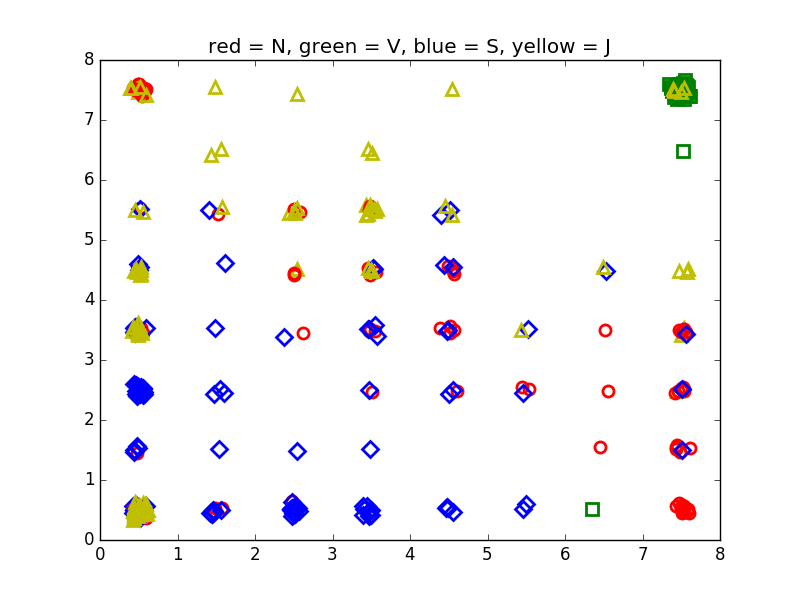
\includegraphics[width=9cm]{../out/CoolResults/som_weights.png}
	\caption{Resultados de una red SOM sobre algunos datos}
	\label{fig_som}
\end{figure}

\section{Posibles Mejoras}

Se podr\'{i}a implementar el m\'{e}todo denominado como \textit{Cascade Correlation} (Fahlman et al. 1990) que permite ajustar din\'{a}micamente la estructura de la red. La misma comienza con una red minimalista (perceptr\'{o}n simple) y luego va ajustando los nodos de la capa oculta durante el entrenamiento.

El dropout prob\'{o} ir reduciendo el error cuadr\'{a}tico medio, sin embargo se podr\'{i}a realizar m\'{a}s mediciones para encontrar el valor \'{o}ptimo del mismo ya que solo se iter\'{o} con 5 posibles valores y realizando mayor cantidad de mediciones podr\'{i}a encontrarse un valor que mejor represente los datos. Tambi\'{e}n, se utiliz\'{o} el test set para verificar los errores siempre igual y con 100 ejemplares de cada categor\'{i}a. Se podr\'{i}an variar estos par\'{a}metros para verificar la estabilidad de los resultados frente a distintos test sets.

Se deber\'{i}a seleccionar los datos de entrenamiento de una forma que asegure que los mismos no se repitan. Adem\'{a}s se podr\'{i}a usar un set de entrenamiento con una cantidad distinta para cada categor\'{i}a en relaci\'{o}n a su cantidad de latidos en el set de datos y verificar como se modifican los resultados con ello (que aspectos se mejoran y cuales no).

La librer\'{i}a permite definir funciones costo propias. \'{E}sto se podr\'{i}a aprovechar para definir una funci\'{o}n de costo propia que le otorgue menor peso a los casos Normales respecto a los dem\'{a}s.

La librer\'{i}a ofrece muchas variantes de backpropagation que no fueron probadas ni investigadas. Ser\'{i}a interesante inspeccionar sobre dichas variantes.

Ser\'{i}a interesante eliminar los Nodales Prematuros y considerar solo los otros tres casos. Los resultados obtenidos con SOM parecen indicar que los mayores problemas derivan por los mismos por lo que quiz\'{a}s mejore mucho la eficiencia de la red si solo se trabajara con 3 categor\'{i}as.

\IEEEpeerreviewmaketitle

\newpage

\IEEEtriggeratref{8}
\bibliographystyle{IEEEtran}
\bibliography{ref}
\end{document}